\subsection{hypothèse et }

Pour étudier caractère pseudo-aléatoire du premier million de décimales de $e$ , nous avons effectué des tests d'hypothèses. L'hypothèse nulle $H_0$ : "Les décimales suivent une loi uniforme" et une hypothèse alternative $H_1$ : "Les décimales ne suivent pas une loi uniforme". Afin de déterminer si l'hypothèse nulle est raisonnable, nous avons représenté les résultats pour ces deux tests ci-dessous:

\begin{figure}[!h]
    \centering
    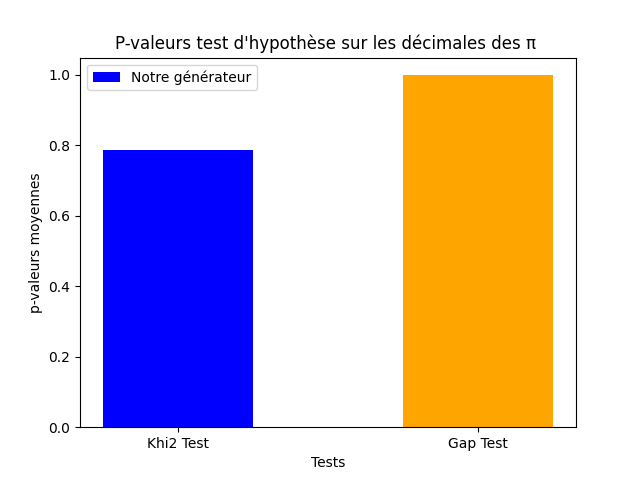
\includegraphics[scale=0.5]{rapport/images/fig/FigDecPi.png}
    \caption{Histogramme de test des décimales}
    \label{enter-label}
\end{figure}
\\

  les valeurs numériques correspondant au graphique ci-dessus.

\begin{table}[!h]
    \centering
    \begin{tabular}{ccc}
        \hline
        Tests & p-valeurs & $\chi^2_{cal}$ \\
        \hline
        $\chi^2$ & 0.787 & 5.51  \\
        Gap & 0.999 & 83.2 \\
        \hline

    \end{tabular}
    \caption{Résultats numériques des tests sur les décimales}

\end{table}
